% Brilliant documentation:
% http://mirror.ox.ac.uk/sites/ctan.org/macros/latex/contrib/beamer/doc/beameruserguide.pdf

\usepackage{beamerthemesplit}
\usepackage{tikz}
\usetikzlibrary{arrows.meta,shapes,backgrounds,positioning,shapes.multipart}
\usepackage{textpos} 
\usepackage{hyperref}
\usepackage{graphicx}
\usepackage{calc}
\usepackage{changepage}
\mode<article>{\usepackage{fullpage}}
\newlength{\popupimagewidth}

\setlength{\popupimagewidth}{\textwidth*3/5}

\putlogoinslide
\newcommand{\defineterm}[2]{\textbf{#1} -- #2}
\newcommand{\geek}{\leavevmode\marginpar{\raisebox{-.35\height}{
\includegraphics[height=5mm,width=5mm]{geek.png}}} }

\newcommand{\startslide}{}
\newcommand{\slideend}{}
%\newcommand{\startslide}{\noindent\hrulefill\ \textit{Start of slide} \\}
%\newcommand{\slideend}{\noindent\hrulefill\ \textit{End of slide} \\}
% Attempt to define new environment for frames that puts a line above and below the frames in the article.
% Unfortunately, this seems to cause the frames to be missed out of the presentation!
%\newcounter{FrameNumber}
%\newenvironment<>{myframe}[2][]
%{\stepcounter{FrameNumber} 
%\hrulefill \ Slide \theFrameNumber
%\begin{frame}[#1]
  %\frametitle{\theFrameNumber. #2}}
%{\end{frame}
%\hrulefill \ End of Slide \theFrameNumber}

\title{Linked Open Data for the Solidarity Economy}
\author{Matt Wallis}
%\date{\today}
\date{February 17, 2017}

% From http://tex.stackexchange.com/a/183966:
\tikzset{
    invisible/.style={opacity=0,text opacity=0},
    visible on/.style={alt=#1{}{invisible}},
    alt/.code args={<#1>#2#3}{%
      \alt<#1>{\pgfkeysalso{#2}}{\pgfkeysalso{#3}} % \pgfkeysalso doesn't change the path
    },
}

\begin{document}
\maketitle
This handout is to accompany the presentation at the Open:2017 conference,
and contains all of the slides from Matt's presentation.
It also contains some additional notes --
some of the notes are quite geeky, and these can be skipped. They can be identified by the geek in the right margin, as seen below.

\geek There are two types of people in the world -- those who can extrapolate from incomplete data.

\startslide
\begin{frame}{Before we start}
  \begin{center}
    A handout to accompany this talk is \textbf{available now}:

    %Short URL:
    \url{http://bit.do/open2017-data-handout}

    %Full URL:

    %\url{http://solidarityeconomics.org/resources/Open2017-data-handout.pdf}

	  \vspace{1cm}
    Twitter: \href{https://twitter.com/SolidarityEcon}{@SolidarityEcon}
  \end{center}
\end{frame}
\slideend
\frame{\titlepage}

\frame{\tableofcontents}

\section{Institute for Solidarity Economics}
\subsection{Who we are}
\startslide
\frame
{
  \frametitle{Institute for Solidarity Economics}
  \begin{center}
    
\includegraphics[height=2cm,width=2cm]{ise-logo.jpg}
  \end{center}
  \begin{itemize}
    \item<1-> \url{http://solidarityeconomics.org}
    \item<1-> Our aim is to support the Solidarity Economy movement through education, research, and finding opportunities for collaboration.
    \item<2-> The Solidarity Economy is a grassroots movement that is building a fair and ecological alternative to Capitalism.
    \item<3-> We are sponsoring Open:2017
    \item<3-> Find out more in latest edition of STIR magazine
  \end{itemize}
}
\slideend
The Institure for Solidarity Economics is sharing a table with STIR magazine at Open:2017. 
Come and talk to us there.

\subsection{Why data?}
\startslide
\frame
{
  \frametitle{Why data?}
  \begin{itemize}
    \item<1-> Data fuels the World Wide Web
    %\item Valueable because it's essential
    \item<2-> Geographic maps
      \begin{itemize}
	\item Make the Solidarity Economy visible
	\item Every map needs data
      \end{itemize}
    \item<3-> Apps to support the movement
      \begin{itemize}
	\item Every app needs data
      \end{itemize}
    \item<4-> Fits our aims: research, education, collaboration
    \item<4-> Starting point:
      \begin{itemize}
	\item Data to describe initiatives in the Solidarity Economy
      \end{itemize}
  \end{itemize}
}
\slideend
\startslide
\frame
{
  \frametitle{Guiding Principles 1: Social}
  \begin{itemize}
    \item<1-> Data ownership is power - be careful!
    \item<2-> Prefer distributed data to centralized data
    \item<2-> Prefer appropriate ownership of data
      \begin{itemize}
	\item Links are better than copies
	  \only<article> {For example, consider weather forecasts --
	  A copy of a weather forecast gets out of date!
	  A link is much better -- let the Met Office own the data.}
      \end{itemize}
    \item<3-> Trust is vital - make sources of data visible
    \item<article> We are all familiar with the power wielded by the big corporations who dominate data.
      We want a solution that permits the data to be owned by the people whose resources are described by that data.
      They may choose to allow someone else to own it, but we want to give them that choice.
  \end{itemize}
}
\slideend
\section{What we did}
\subsection{Research and Development}
\startslide
\frame
{
  \frametitle{Guiding Principles 2: Engineering}
  \begin{itemize}
    \item<1-> Use existing best practice
    \item<1-> Re-use existing software
    \item<1-> Re-use existing data (link, don't copy!)
    \item<1-> Re-use existing data models
    \item<2-> Open source
      \begin{itemize}
	\item Use open source software
	\item ISE publishes work with open source licenses
      \end{itemize}
  \end{itemize}
}
\slideend
\startslide
\frame
{
  \frametitle{Research}
  \begin{itemize}
    \item<1-> Linked Open Data (LOD) looked like best practice
    \item<1-> But scary! {\em we needed to understand it better}
    \item<2-> Experimentation and discovery
      \begin{itemize}
	\item Publish a dataset using LOD principles
	\item Use that dataset in an app
      \end{itemize}
  \end{itemize}
}
\slideend
\startslide
\frame
{
  \frametitle{Development}
  \begin{itemize}
    \item Generated experimental LOD dataset of over 13,000 UK Co-ops
    \item Deployed the LOD dataset - openly available on the web
    \item Put the 13,000 co-ops on a map
    \item Document and educate
  \end{itemize}
}
\slideend
Our work is available on GitHub: \url{https://github.com/p6data-coop/ise-linked-open-data}
We used the existing ESSGLOBAL vocabulary for Linked Open Data.

\subsection{Map of UK co-ops}
\startslide
\frame
{
  \frametitle{map-app}
  \begin{itemize}
    \item<1-> Web application to show UK co-ops on a map
    \item<2-> Data is loaded from our Linked Open Database
    \item<3-> map-app provides links to LOD that is provided by others
      \begin{itemize}
	\item<3-> Ordnance Survey
	\item<3-> Companies House
      \end{itemize}
    \item<4-> map-app links to educational material about our LOD
    \item<article> Clean separation of application and data
  \end{itemize}
}
\slideend

You can take a look at the map-app by clicking on the link: \url{http://data.solidarityeconomics.org/map-app/}.
Please note that if lots of people do this at the same time during the presentation, it will be slow to load, because the data is hosted on a very small server.

The map-app was developed for two main reasons:
  \begin{itemize}
    \item An experimental platform to help us during development
    \item An educational aid to see linked open data in action 
  \end{itemize}

\subsection{Linked Open Data}
\startslide
\frame
{
  \frametitle{Links to the webs}
  \begin{center}
    \makebox[\textwidth]{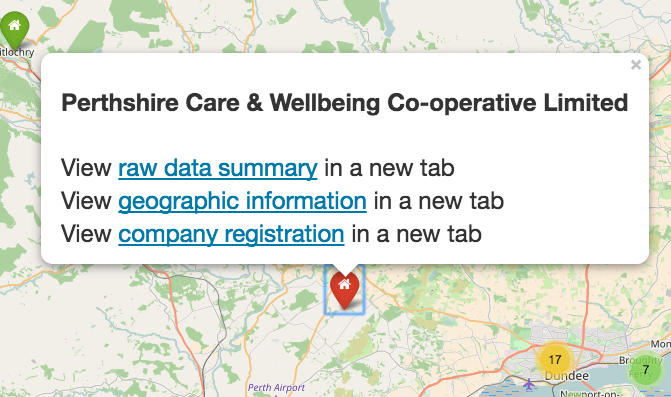
\includegraphics[width=\popupimagewidth]{map-app-popup-screenshot.png}}
  \end{center}
  \begin{itemize}
    \item Web of Documents
    \item Web of Data
  \end{itemize}
}
\slideend
By clicking on a marker on the map-app, a pop-up will appear, as shown above.
Only the red markers have links to data held by Companies House.

\subsection<article>{Links}

Some of the links that are displayed in the pop-up are links to two different World Wide Webs: the \textit{Web of Documents} and the \textit{Web of Data}.
The Web of Documents is the one that we are all familiar with; it is the place we inhabit through web browsers, and was designed to deliver documents for humans to read.
The Web of Data shares the same infrastructure (the internet, web servers, etc) as the Web of Documents, but it allows machines to request machine-readable data instead of human-readable documents.

\geek By clicking the \textbf{raw data summary} link, your browser will take you to a page in the Web of Documents that shows data for a co-op. 
That page is identified by a URI (Uniform Resource Identifier) that looks just like a URL (Uniform Resource Locator) you might see in your browser's URL bar. For example:

{\footnotesize \url{http://data.solidarityeconomics.org/id/experimental/test/co-ops-uk/R005512}}

\geek When a web browser requests a URI, the web server will redirect the browser to a page in the Web of Documents that has the following URL:

{\footnotesize \url{http://data.solidarityeconomics.org/doc/experimental/test/co-ops-uk/R005512.html}}

\geek But, when a machine requests that same URI, the web server will redirect the machine to data in the Web of Data. 
The machine can request a number of different data formats from the web server.
If the machine requested the Turtle data format, then the web server will redirect it to this URL:

{\footnotesize \url{http://data.solidarityeconomics.org/doc/experimental/test/co-ops-uk/R005512.ttl}}

\geek The machine-readable data in the Turtle format looks like this:

%\vspace{1cm}
%\begin{adjustwidth}{-2cm}{0pt}
{\footnotesize
\begin{verbatim}
@prefix essglobal: <http://purl.org/solidarityeconomics/experimental/essglobal/vocab/> .
@prefix gr: <http://purl.org/goodrelations/v1#> .
@prefix ospostcode: <http://data.ordnancesurvey.co.uk/id/postcodeunit/> .
@prefix osspatialrelations: <http://data.ordnancesurvey.co.uk/ontology/spatialrelations/> .
@prefix rdf: <http://www.w3.org/1999/02/22-rdf-syntax-ns#> .
@prefix rov: <http://www.w3.org/ns/regorg#> .
@prefix vcard: <http://www.w3.org/2006/vcard/ns#> .
@prefix xsd: <http://www.w3.org/2001/XMLSchema#> .

<http://data.solidarityeconomics.org/id/experimental/test/co-ops-uk/R005512> a essglobal:SSEInitiative;
   gr:name "Pant-yr-Athro Park Management Company";
   essglobal:hasAddress <http://data.solidarityeconomics.org/id/experimental/test/co-ops-uk/R005512Address>;
   essglobal:legalForm <http://purl.org/solidarityeconomics/experimental/essglobal/standard/legal-form/L2>;
   rov:hasRegisteredOrganization <http://business.data.gov.uk/id/company/01113761> .

<http://data.solidarityeconomics.org/id/experimental/test/co-ops-uk/R005512Address> a essglobal:Address;
   osspatialrelations:within ospostcode:SA335AJ;
   vcard:country-name "UK";
   vcard:postal-code "SA33 5AJ" .
\end{verbatim}
}
%\end{adjustwidth}

%\frame[fragile,t]
%\frame[t]
\startslide
\begin{frame}[t]
  \frametitle{The data are links}
  \centering
  %\begin{center}
  %\begin{tikzpicture}[scale=.8, show background rectangle, node distance=1cm]
  %\begin{tikzpicture}[remember picture, show background rectangle, node distance=1cm]
  \begin{tikzpicture}[remember picture, node distance=1cm]
    \tikzstyle{every text node part} = [align=center]
    \tikzstyle{obj node} = [ellipse, fill=blue!20]
    \tikzstyle{obj path} = [->, draw=blue!20]
    \tikzstyle{label node} = [draw, text=black]
    \tikzstyle{data node} = [rectangle, fill=green!20]
    \tikzstyle{extdata node} = [rectangle, draw, fill=green!20]
    \tikzstyle{app node} = [rectangle, fill=red!20]
    \tikzstyle{label node} = [midway, auto]
    \tikzstyle{label text} = [align=left]
    \node[obj node] (iseobj) {\underline{Links to other datasets} e.g. \\ {\visible<2->{http://os.gov/postcode/SA335AJ}} \\ {\visible<3->{http://ch.gov/company/01113761}}};
    \node[label text, visible on=<1->] (datalabel) [left = of iseobj] {Example \\ data:};
    \node[extdata node, visible on=<2->] (osdata) [below = of iseobj ] {OS data};
    \node[data node] (isedata) [left = of osdata] {Our data};
    \node[extdata node, visible on=<3->] (chdata) [right = of osdata] {CH data};
    \node[label text, visible on=<1->] (datasetlabel) at (isedata-|datalabel) {Datasets:};

    \node[app node, visible on=<4->] (mapapp) [below left = of osdata] {Map};
    \node[app node, visible on=<5->] (nearestapp) [below right = of osdata] {Nearby};
    \node[label text, visible on=<4->] (appslabel) at (mapapp-|datasetlabel) {Apps:};
    \draw[->, visible on=<1->] (isedata) -- (iseobj) node[label node]{contains};
    \draw[->, visible on=<2->] (iseobj) -- (osdata) node[midway, left]{link};
    \draw[->, visible on=<3->] (iseobj) -- (chdata) node[midway, right]{link};
    \draw[<->, visible on=<4>] (mapapp) -- (isedata) node[midway, right]{query};
    \draw[<->, visible on=<4>] (mapapp) -- (osdata) node[midway, right]{query};
    \draw[->, visible on=<5->] (mapapp) -- (nearestapp) node[midway, below]{http://ch.gov/...};
    \draw[<->, visible on=<5->] (nearestapp) -- (osdata) node[midway, left]{query};
    \draw[<->, visible on=<5->] (nearestapp) -- (chdata) node[midway, right]{query};
  \end{tikzpicture}
    \begin{itemize}
      \item<3-> Existing data: CH = Companies House
      \item<2-> Existing data: OS = Ordnance Survey
    \end{itemize}
  \end{frame}
    \slideend

In the picture above \dots
    \begin{description}
      \item[Our data]is the Linked Open Data we created to describe the 13,000 co-ops.
      \item[OS data] is Linked Open Data published by Ordnance Survey.
      \item[CH data] is Linked Open Data published by Companies House.
      \item[http://os.gov/postcode/OX10AB] \geek represent the proper URI \url{http://data.ordnancesurvey.co.uk/id/postcodeunit/SA335AJ}
      \item[http://ch.gov/company/01113761] \geek represents the proper Companies House URI \url{http://business.data.gov.uk/id/company/01113761}
      \item[Nearby] is the application that is launched when ``similar companies nearby'' is clicked in the map-app. 
	It makes use of both the OS data and the CH data:
	The OS data can tell us which postcodes are within a particular geographics area, and the CH data can tell us what line of business a company is in.
	Putting these two together, we can ask for all the companies that are in the same line of business, and in the same geographics area as a particular company.
	For example, the map-app passes the detail of a co-op to the Nearby application, and it displays all companies that are in the same line of business and same geographical area as that co-op.
      \item[http://ch.gov/...] \geek is a link to Companies House that is passed as data to the Nearby application.
    \end{description}

\section{Conclusions}
%\frame
%{
  %\frametitle{Lessons from re-use}
  %\begin{itemize}
    %\item Makes the original developers very happy
    %\item Great co-operation from original developers
    %\item Learn from others
    %\item Answers questions you'd not know to ask \texttt{!important;}
    %\item Leave things in better shape
  %\end{itemize}
%}
\startslide
\frame
{
  \frametitle{LOD Everywhere? No}
  \begin{center}
    %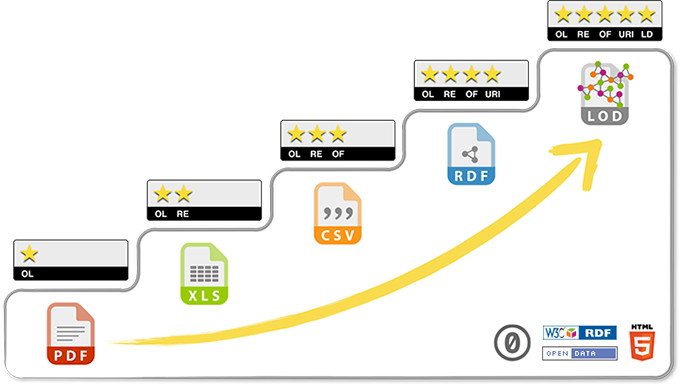
\includegraphics{5-star-steps.png}
    \makebox[\textwidth]{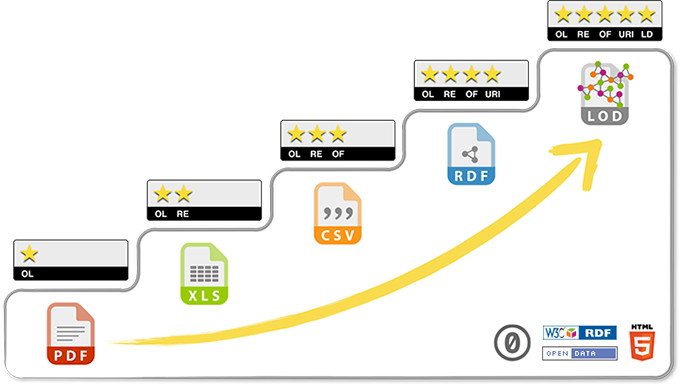
\includegraphics[width=\popupimagewidth]{5-star-steps.png}}
    %\makebox[\textwidth]{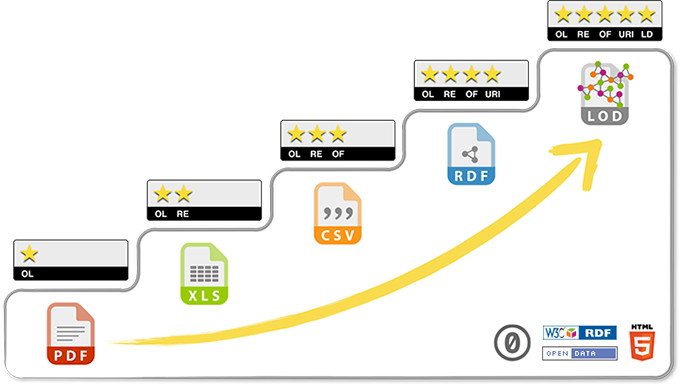
\includegraphics[width=\paperwidth]{5-star-steps.png}}
    %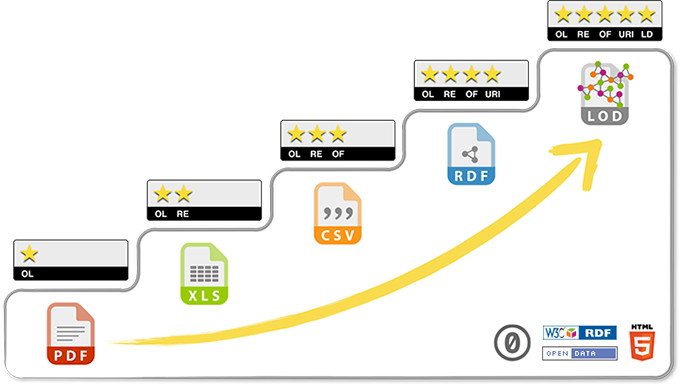
\includegraphics[height=2cm,width=2cm]{5-star-steps.png}
  \end{center}
  \begin{itemize}
    \item \url{http://5stardata.info}
  \end{itemize}
}
\slideend
The descriptions of the 5 star classifications at \url{http://5stardata.info} are both brief and informative.
\startslide
\frame
{
  \frametitle{The LOD approach}
  \begin{itemize}
    \item<1-> Answers question you didn't even know to ask!
    \item<1-> Enables appropriate ownership of data
    \item<2-> Semantic data modelling is very powerful
    \item<2-> Technically, ticks the boxes
      \begin{itemize}
	\item Interoperability
	\item Global identifiers (http links)
	\item Harnesses existing power of the Web of Documents
	\item Easily integrate with other data standards
	\item \dots
      \end{itemize}
    \item<3-> Highly knowledgeable and helpful online community
    \item<4-> Excellent for ``National Grid'' of data
  \end{itemize}
}
\slideend
\begin{description}
  \item[Appropriate ownership] Ordnance Survey owns geographics data; Companies House owns company registration data; Data about the Solidarity Economy can be distributed.
  \item[Semantic data modelling] \geek Consider postcodes. SA33 5AJ is within SA33 5; SA33 5 is within SA 33; SA33 is within SA. From the semantics of the data model, we can infer that SA33 5AJ is therefore within SA. This just touches the surface of the power of semantic data modelling.
  \item[National Grid of data] This analogy with the electricity grid is about building fundamental infrastructure.
  \item[Harness Web of Documents] \geek Why invent new ways of dealing with data when these can be re-used from the Web of Documents? e.g. HTTP, global URI namespace, web servers, content negotiation to provide data is a wide range of formats, \dots
\end{description}
\startslide
\frame
{
  \frametitle{What's next?}
  \begin{itemize}
    \item Talk to us about Linked Open Data
    \item Talk to us about other datasets
  \end{itemize}
}
\slideend

\subsection<article>{Links to more on LOD}
Here are a few links to provide more information about Linked Open Data:

  \begin{itemize}
    \item Tim Berners-Lee talking at TED2009: \url{https://www.ted.com/talks/tim_berners_lee_on_the_next_web}
    \item Video by Europeana: \url{https://vimeo.com/36752317}
    \item \url{http://linkeddata.org/}
    \item \url{https://www.w3.org/standards/semanticweb/data}
    \item Getting into technical detail: \url{http://linkeddatabook.com/editions/1.0/}
  \end{itemize}


\end{document}
